% Body-only English translation draft.
% The Korean source and its internal editorial memo remain authoritative:
% ../Full_Paper_Draft_ko.md
% Appendices and references are intentionally omitted at this migration stage.
\documentclass[letterpaper]{article}

\usepackage[submission]{aaai2027}
\usepackage[hyphens]{url}
\usepackage{graphicx}
\urlstyle{rm}
\def\UrlFont{\rm}
\usepackage{natbib}
\usepackage{caption}
\usepackage{booktabs}
\usepackage{algorithm}
\usepackage{algorithmic}
\usepackage{amsmath}
\usepackage{amssymb}
\frenchspacing

\setcounter{secnumdepth}{2}

\pdfinfo{
/TemplateVersion (2027.1)
}

\title{StreamWeave: Reconciling Off-Policy Expert Supervision with Fully-Asynchronous Policy Learning}

\author{Anonymous Submission}
\affiliations{}

\begin{document}
\maketitle

\begin{abstract}
Reinforcement learning with verifiable rewards (RLVR) spends substantial generation work on long rollouts for problems that the policy cannot yet solve, but obtains no group-relative learning signal when every response to a prompt fails.
Fully-asynchronous RL reduces execution cost by overlapping rollout generation with model training, while expert trajectories provide solution paths where policy-generated signal is absent.
In the group-conditioned setting studied here, however, the outcome of a complete group determines both the training source and the learning role of each sample, whereas a fully-asynchronous runtime executes trajectory attempts independently.
Our key insight is that a complete group can remain the boundary of a learning decision without making its completion a pipeline-wide execution barrier.
StreamWeave executes attempts independently, reconstructs a complete group at the source-decision boundary, and converts the resolved source and generation context into the corresponding training input.
Policy and expert inputs are then consumed in one primary update with one policy objective and the same averaging rule, while rollout generation and model training remain concurrent.
On mathematical reasoning benchmarks, StreamWeave achieves an average score of 38.5, comparable to 37.7 for a synchronous quality reference that uses the same group-success selector.
It also reduces the processing time for 128 prompt groups from 46 to 28 seconds and improves prompt-group throughput by $1.64\times$ under the same GPU budget.
StreamWeave preserves group-conditioned heterogeneous learning while realizing the efficiency of fully-asynchronous execution in one training system.
\end{abstract}

\section{Introduction}
\label{sec:introduction}

Reinforcement learning with verifiable rewards (RLVR) improves the reasoning ability of large language models by reinforcing automatically verifiable successes.
On problems that the policy cannot yet solve, however, it may spend substantial generation work without obtaining a learning signal.
Group-based RLVR generates multiple rollouts from the same prompt to search for a correct solution, and long reasoning trajectories make this generation a major part of training wall-clock time.
When every rollout in the group fails, the reward contrast within the group vanishes, leaving no relative learning signal.
In our training trace, all-failure groups account for 22.4\% of all groups but 26.8\% of generated response tokens.
Computational burden and signal scarcity therefore concentrate in the same hard region.
Fully-asynchronous RL reduces the execution bottleneck by overlapping rollout generation with model training, while methods that use expert trajectories provide external solution paths for problems that the policy fails to solve.
Scaling group-conditioned RLVR needs both capabilities, but combining them does not by itself determine how a decision defined on a complete group reaches a runtime built to advance attempts independently.

The two capabilities interact directly because a complete-group outcome now does more than support a relative signal: a group containing a success learns from policy rollouts, whereas an all-failure group selects the paired expert trajectory.
The group therefore determines both the training source and how the selected samples contribute to the update.
Fully-asynchronous execution gains efficiency by running trajectory attempts from the same group independently.
Treating a complete group as the execution unit places its slowest trajectory on the pipeline critical path, while losing source identity would erase the distinct learning roles of policy and expert samples.
The central challenge is to carry a complete-group decision into an asynchronous training stream without binding trajectory execution back into groups.
We therefore ask: \textbf{Can a system preserve complete-group decisions while retaining trajectory-level fully-asynchronous execution?}

\begin{figure*}[t]
  \centering
  
\includegraphics[width=0.94\textwidth]{figure1.pdf}
  \caption{The wait for one complete group is local.
  While a group is still incomplete, other rollout generation and already-prepared training continue; an all-failure group then selects the expert source and a group containing a success keeps its policy rollouts.}
  \label{fig:scoped-dependencies}
\end{figure*}

Figure~\ref{fig:scoped-dependencies} summarizes how StreamWeave bounds the two dependencies required by this learning program.
It executes trajectory attempts independently, reconstructs a complete group only for its source decision, and carries the resolved source and generation context across the queue in one training record.
The record is then converted into the input required by that source, allowing the Generator to continue producing trajectories while the learner consumes prepared inputs.
The complete group remains the learning-decision boundary without propagating its completion wait to other rollout generation or model training.

This handoff also preserves the learning roles of the two sources.
The decision fixes the sequence, signal, ratio reference, and policy-lag correction represented by the training input.
Policy and expert inputs then enter one primary update with one policy objective and the same averaging rule, reducing respectively to group-relative reinforcement and supervised learning.
StreamWeave thus confines the required coupling to complete-group decision and training-input construction while leaving the rest of the pipeline open to trajectory-level asynchrony.

Experiments on mathematical reasoning show that StreamWeave reaches an average score of 38.5, competitive among the evaluated RL and expert-trajectory methods and comparable to the 37.7 achieved by a synchronous quality reference with the same group-success selector.
The learning dynamics further show that the hard region requiring expert trajectories persists late into training, and that the performance of StreamWeave and an expert-off control separates as training proceeds.
StreamWeave sustains this online expert channel even under the longer generation workload observed when expert inputs are used.
It reduces the processing time for 128 prompt groups from 46 to 28 seconds and increases prompt-group throughput by $1.64\times$ under the same GPU budget.
Together, these results show that group-conditioned learning composition and fully-asynchronous execution can be realized in one training system.

A complete-group decision imposes two requirements whose lifetimes differ.
The execution that waits for the group ends once its source is fixed, whereas the information that reproduces the learning role selected by that source must survive until the training input is built.
StreamWeave ends each requirement where it is consumed, and our contributions follow that division:
\begin{itemize}
  \item \textbf{Asynchrony-compatible learning composition.}
  We identify what a resolved source must carry forward for the learner to reproduce the role it selects: the source itself, the reward context of its group, and the generation policy of each rollout.
  These are expressed as the training input each source requires, and once that input exists no source-specific decision remains in the learner or optimizer path, so both sources share one policy objective and the same averaging rule.
  A constructive derivation shows that the two inputs reduce to their intended group-relative and supervised contributions.

  \item \textbf{Boundary-localized asynchronous architecture.}
  We execute trajectory attempts independently, reconstruct the complete group only before its source decision, and preserve the resolved source and generation context until training-input construction.
  By placing the required processing at the boundaries of the asynchronous queue, StreamWeave retains the basic roles of the Generator and learner and confines complete-group waiting to the source decision.

  \item \textbf{Composition-aware empirical study.}
  We measure how generation work concentrates where successful policy signal is scarce, how the demand for expert trajectories persists through training, and how expert supervision changes the asynchronous workload.
  Under these conditions, StreamWeave jointly achieves competitive reasoning performance and $1.64\times$ prompt-group throughput under the same GPU budget.
\end{itemize}

\section{Related Work}
\label{sec:related-work}

StreamWeave connects two lines of work: systems that decouple rollout generation from model training and methods that learn from expert data outside the policy's own rollouts.
The former addresses execution efficiency, while the latter addresses the absence of policy-generated signal.
StreamWeave studies their composition when the outcome of a complete group also determines the training source.

\paragraph{Fully-asynchronous policy learning.}
HybridFlow~\citep{sheng2025hybridflow} separates computation and data dependencies in RLHF, providing an execution substrate for flexible algorithms and resource mappings.
Asynchronous RLHF~\citep{noukhovitch2025asyncrlhf} directly decouples generation from learning and studies the trade-off between execution efficiency and policy lag when training on samples from earlier policies.
AReaL~\citep{fu2025areal} fully disaggregates rollout and training workers and combines workload balancing with staleness-aware optimization in an end-to-end asynchronous LLM RL system.
TBA~\citep{bartoldson2025tba} trains an off-policy objective on replay experience collected by asynchronous actors.
Laminar~\citep{sheng2026laminar} independently executes trajectories in GRPO to absorb variation in generation latency within a group.
These systems decouple the production and consumption of policy-generated rollouts while controlling the resulting policy lag.

\paragraph{Learning from policy rollouts and expert trajectories.}
A second line of work extends learning beyond experience generated by the current policy through demonstrations, offline data, or expert trajectories.
In general reinforcement learning, DQfD~\citep{hester2018dqfd} uses demonstrations in temporal-difference updates and a supervised loss, while RLPD~\citep{ball2023rlpd} continually incorporates offline data into online RL.
In LLM post-training, InstructGPT~\citep{ouyang2022instructgpt} stages demonstration-based supervised learning before RLHF, and SimpleMix~\citep{li2025simplemix} directly mixes on-policy and off-policy data for preference learning.
For reasoning post-training, LUFFY~\citep{yan2025luffy} combines off-policy reasoning traces with policy rollouts through mixed-policy learning.
CHORD~\citep{zhang2026chord} reformulates SFT as a dynamically weighted auxiliary objective optimized alongside on-policy exploration.
ReLIFT~\citep{ma2026relift} and SRFT~\citep{fu2026srft} also use expert trajectories for reasoning post-training.
This line of work has developed methods for selecting external data and assigning a learning role and weight to each source.

\paragraph{Composing asynchronous execution with heterogeneous supervision.}
Combining these lines requires converting a complete-group decision into a training record that an asynchronous stream can consume.
The group outcome chooses between policy rollouts and an expert trajectory, and the chosen source changes both the sequence used for learning and the conditions of its training input.
Neither line determines how far the wait for that outcome should reach, nor how long the selected source and its group context must remain available.
A system whose groups carry no consequence for the learning signal never faces the first question, and a synchronous barrier that holds every sequence until the update answers the second by default.

\section{StreamWeave}
\label{sec:method}

StreamWeave separates three units: trajectory attempts for execution, complete prompt groups for learning decisions, and source-appropriate training inputs for optimization.
Attempts execute independently; when a group completes, it selects either the policy group or its paired expert trajectory.
Cross-attempt waiting ends once the source is fixed, while the source and required group context persist until input construction.
Outside this handoff, the Generator continues rollout generation and the learner updates prepared inputs.
Section~\ref{sec:learning-composition} asks what a complete-group decision must carry forward for the learner to reproduce the role it selects.
Section~\ref{sec:async-execution} asks how far the execution that waits for that decision has to reach.
Figure~\ref{fig:data-state-boundaries} shows the three data-state boundaries at the queue handoff, and Algorithm~\ref{alg:streamweave} summarizes the concurrent control flow.

\begin{figure*}[t]
  \centering
  
\includegraphics[width=0.94\textwidth]{figure2.pdf}
  \caption{StreamWeave's three data-state boundaries under the $\gamma=0$ source rule.
  A complete group becomes either an $n$-sequence policy record or a singleton expert record; both share one queue, are converted to source-appropriate inputs, and enter one primary update.
  Policy provenance enables rollout-to-entry correction, whereas expert input uses identity correction.}
  \label{fig:data-state-boundaries}
\end{figure*}

\subsection{Learning Composition}
\label{sec:learning-composition}

A complete-group decision fixes more than which sequence to train on: it fixes the conditions under which the learner interprets that sequence.
This section identifies what such a decision must carry forward, expresses it as the training input each source requires, and shows that both inputs then enter one policy objective with the same averaging rule.
Our experiments instantiate the source rule with Hybrid Post-Training (HPT)~\citep{lv2025hpt}, which selects between a policy group and an expert trajectory from the outcome of a complete rollout group.

\paragraph{Source selection from a completed group.}
For prompt $x$, let
$G_x=\{\tau_{x,1},\ldots,\tau_{x,n}\}$
denote $n$ policy-generated rollouts.
Each rollout has verifier score $R(\tau_{x,i})$, and the success rate of the complete group is
\begin{equation}
\begin{aligned}
P_x &=
\frac{1}{n}\sum_{i=1}^{n}
\mathbf{1}\!\left[R(\tau_{x,i})>\delta\right],\\
z_x &= S_\gamma(G_x)=
\begin{cases}
\mathrm{expert}, & P_x\le\gamma,\\
\mathrm{policy}, & P_x>\gamma.
\end{cases}
\end{aligned}
\label{eq:source-selection}
\end{equation}
Training uses the generated group $G_x$ when $z_x=\mathrm{policy}$ and the expert trajectory $\tau_x^\star$ paired with the same prompt when $z_x=\mathrm{expert}$.
Because the decision is defined on the outcome of $G_x$ rather than on any individual trajectory, the source can be resolved only after all $n$ verifier scores have arrived.
Section~\ref{sec:experimental-setup} specifies $n$, $\gamma$, and the coverage of expert trajectories.

\paragraph{Constructing source-specific training inputs.}
The source decision determines not only the sequence used for learning, but also how its learning signal is formed, which reference defines its policy ratio, and whether policy-lag correction applies.
For token $t$ in selected sequence $r$, let $\ell_{\theta,r,t}$ be its log-probability under the current policy, $A_{r,t}$ the learning signal, $\rho_{r,t}$ the policy ratio, and $w_{r,t}$ the importance weight that corrects the difference between the rollout policy and the policy at update entry.

For the policy source, StreamWeave retains all $n$ rollouts and compares their verifier scores to compute the GRPO advantage~\citep{shao2024deepseekmath} $A^{\mathrm{grp}}_{r,t}$.
A rollout may have been generated by a policy version that predates the update.
We therefore use the policy at update entry as the ratio reference and account for the lag from generation through a separate weight:
\begin{equation}
\begin{aligned}
A_{r,t} &= A^{\mathrm{grp}}_{r,t},
& w_{r,t} &= w^{\mathrm{lag}}_{r,t},\\
\rho_{r,t}
&= \exp\!\left(
\ell_{\theta,r,t}-\ell^{\mathrm{entry}}_{r,t}
\right).
\end{aligned}
\label{eq:policy-input}
\end{equation}

An expert trajectory is an externally supplied target sequence rather than past experience generated by the policy.
Its role is therefore to increase the likelihood of the target directly, without a group-relative signal or rollout-to-entry correction.
Using the supervision strength $\beta_r$ as its signal and a stop-gradient copy of the current-policy log-probability as its reference makes the forward ratio equal to one:
\begin{equation}
\begin{aligned}
A_{r,t} &= \beta_r,
& w_{r,t} &= 1,\\
\rho_{r,t}
&= \exp\!\left(
\ell_{\theta,r,t}-\operatorname{sg}[\ell_{\theta,r,t}]
\right)=1.
\end{aligned}
\label{eq:expert-input}
\end{equation}

\paragraph{One policy objective.}
Inputs from both sources enter the same token-level policy objective $\Phi$.
For batch $B$,
\begin{equation}
\mathcal{L}(B)=\frac{1}{|B|C}
\sum_{r\in B}\sum_t m_{r,t}
\Phi\!\left(\rho_{r,t};A_{r,t},w_{r,t}\right),
\label{eq:primary-objective}
\end{equation}
where $m_{r,t}$ is the response mask and $C$ is a normalization constant shared by all sequences.
The policy input produces a group-relative policy contribution.
For the expert input, the forward ratio is one but its numerator retains a gradient, yielding a supervised negative-log-likelihood contribution weighted by $\beta_r$.
Both inputs therefore share one optimizer path, one policy objective, and the same averaging rule.
Our experiments instantiate $\Phi$ with vanilla clipped PPO~\citep{schulman2017ppo}.
Appendices A.2 and A.3 derive the expert endpoint and the shared averaging rule, establishing that the source semantics are fixed during input construction while the objective and aggregation remain common.

The complete-group decision jointly determines the sequence used for learning and how that sequence contributes to the update.
Nothing in this account says how long execution must wait for that decision, which is the question the next section takes up.

\subsection{Fully-Asynchronous Execution}
\label{sec:async-execution}

Fully-asynchronous execution uses independent attempt scheduling, a bounded queue, backpressure, and parameter refresh to keep rollout generation and model training concurrent.
StreamWeave concentrates the composition-specific processing at two boundaries of this handoff: it reconstructs the complete group and resolves the source before the queue, then converts the source-fixed record into the corresponding training input after the queue.
Outside these boundaries, the Generator produces trajectory attempts and the learner applies its existing policy update to prepared inputs.

\begin{algorithm}[t]
\caption{StreamWeave}
\label{alg:streamweave}
\begin{algorithmic}[1]
\REQUIRE Prompt pool $\mathcal{X}$, group size $n$, verifier $R$, source rule $S_\gamma$, expert store $\mathcal{E}$
\STATE Initialize accumulator $\mathcal{A}$ and queue $\mathcal{Q}$
\STATE \textbf{Generator and trainer run concurrently}
\STATE \textbf{Generator:} launch an attempt in each idle rollout slot
\STATE On completion of $(g_x,i)$ under $\pi_i^{\mathrm{gen}}$, store
$\langle\tau_i,R(\tau_i),\pi_i^{\mathrm{gen}}\rangle$ in $\mathcal{A}[g_x][i]$
\STATE Immediately launch the next attempt in the released slot
\IF{$|\mathcal{A}[g_x]|=n$}
  \STATE $G_x\leftarrow\operatorname{ordered\_pop}(\mathcal{A}[g_x])$;
  $z_x\leftarrow S_\gamma(G_x)$
  \STATE Push $\operatorname{SourceRecord}(x,z_x,G_x,\mathcal{E}[x])$ to $\mathcal{Q}$
\ENDIF
\STATE \textbf{Trainer:} dequeue source-fixed records and initialize $B$
\FOR{each record $q$}
  \STATE Add $\operatorname{PolicyInputs}(q)$ if $q$ is policy, otherwise add $\operatorname{ExpertInput}(q)$
\ENDFOR
\STATE $\theta\leftarrow\operatorname{LearnerUpdate}(\theta,\mathcal{L}(B))$; publish $\theta$
\end{algorithmic}
\end{algorithm}

\paragraph{Execute attempts independently and reconstruct each group locally.}
Trajectory attempts from one prompt group execute independently while retaining their group identity and position.
Each completion releases its rollout slot for the next task and enters the accumulator.
Once every attempt has arrived, the accumulator restores the complete group in its original order for the source decision.
Other groups continue generating and ready inputs continue training while this group is incomplete, so the complete-group requirement governs decision availability rather than trajectory execution.

\paragraph{Fix the source before the queue.}
Once the group is complete, StreamWeave applies $S_\gamma$ from Section~\ref{sec:learning-composition} and resolves whether training will use the policy rollout group or the paired expert trajectory.
It sends the resolved source, selected data, and required context through the queue in one prompt-group record: policy records retain complete-group scores and per-rollout generation policies, whereas expert records retain the selected target and its source.
Because the source is fixed before transport, queue consumption order can change update timing but cannot revise the learning decision.

\paragraph{Construct training inputs after the queue.}
The trainer converts each dequeued record into the input defined in Section~\ref{sec:learning-composition}.
Policy records provide the complete-group scores and provenance needed for the GRPO signal and policy-lag correction; expert records provide the target needed for a $\beta$-weighted supervised contribution.
The trainer applies the policy objective and averaging rule from Section~\ref{sec:learning-composition} to both inputs.

\paragraph{Keep one asynchronous flow.}
Source-fixed records remain in the existing queue, backpressure, and parameter-refresh flow, while both inputs share one learner and optimizer path.
Waiting for a complete group ends when the accumulator fixes its source; for the policy route, scores and generation context remain in the record until input construction.
This handoff preserves complete-group decisions and source-specific learning roles without changing the core interfaces of the surrounding asynchronous flow.
Appendix B traces where group context and source identity are consumed and shows how the remaining asynchronous substrate stays on one execution path.

\section{Experiments}
\label{sec:experiments}

We evaluate whether StreamWeave preserves the distinct learning roles of policy rollouts and expert trajectories while jointly achieving learning effectiveness and execution efficiency.
Our experiments ask three questions.
First, does StreamWeave achieve competitive mathematical reasoning performance while retaining cross-domain reasoning?
Second, do signal scarcity and generation work concentrate in the all-failure groups that select expert trajectories, and does selective expert supervision contribute to learning beyond those directly routed prompts?
Third, can StreamWeave process the generation workload and source-dependent training inputs of persistent expert supervision at their required boundaries, improving prompt-group throughput under the same GPU budget without turning complete-group decisions into a pipeline-wide execution barrier?

\begin{table*}[t]
\centering
\begin{tabular}{lrrrrrrr}
\toprule
Model & AIME24 & AIME25 & AMC (83) & MATH500 & Minerva & Olympiad & \textbf{Avg.} \\
\midrule
Base & 6.6 & 3.5 & 31.2 & 43.3 & 10.9 & 24.9 & \textbf{20.1} \\
Instruct & 10.6 & 9.4 & 47.0 & 75.5 & 29.5 & 40.4 & \textbf{35.4} \\
SFT$^{\dagger}$ & 11.7 & 13.2 & 37.8 & 70.6 & 26.8 & 31.3 & \textbf{31.9} \\
RL-only$^{\dagger}$ & 11.8 & 7.7 & 40.2 & 61.8 & 26.8 & 32.0 & \textbf{30.1} \\
Async RL (expert-off) & 12.9 & 7.9 & 44.9 & 75.8 & 28.8 & 39.5 & \textbf{35.0} \\
HPT (sync) & 15.4 & 12.6 & 45.8 & 78.0 & 31.3 & 43.2 & \textbf{37.7} \\
SRFT & 12.3 & 10.4 & 43.0 & 71.6 & 26.1 & 38.4 & \textbf{33.7} \\
ReLIFT & 12.6 & 8.1 & 40.3 & 74.6 & 28.6 & 39.4 & \textbf{34.0} \\
Oat-Zero & \textbf{17.2} & 12.6 & \textbf{49.6} & 73.7 & 30.1 & 38.1 & \textbf{36.9} \\
LUFFY & 15.1 & \textbf{14.0} & 46.0 & 77.5 & 30.0 & \textbf{43.5} & \textbf{37.7} \\
\textbf{StreamWeave} & 16.1 & 13.0 & 47.0 & \textbf{78.5} & \textbf{33.0} & 43.2 & \textbf{38.5} \\
\bottomrule
\end{tabular}
\caption{Fixed-checkpoint mathematical reasoning.
Scores are rounded to one decimal; Avg.\ is the unweighted mean of unrounded scores.
$^{\dagger}$Source-reported result.}
\label{tab:math-reasoning}
\end{table*}

\subsection{Experimental Setup}
\label{sec:experimental-setup}

\paragraph{Training setting and control.}
StreamWeave starts from Qwen2.5-Math-1.5B~\citep{yang2024qwen25math} and trains on prompts paired with verified expert trajectories from OpenR1-Math~\citep{huggingface2025openr1}.
For each prompt, the policy generates $n=8$ rollouts.
We set the complete-group source threshold to $\gamma=0$, so the paired expert trajectory is used only when all eight policy rollouts fail.
To isolate the role of the expert channel and the accompanying generation workload, we compare against Async RL (expert-off), which disables the use of expert trajectories while retaining the same fully-asynchronous execution stack.
We refer to it as the expert-off control below.
Appendices A.2--A.4 and C.1 specify the expert-signal scale, asynchronous correction, loss averaging, and optimization configuration.

\paragraph{Reasoning evaluation.}
We perform fixed-checkpoint evaluation on six mathematical reasoning benchmarks: AIME24, AIME25, AMC (83 problems), MATH500~\citep{hendrycks2021math,lightman2024prm800k}, Minerva~\citep{lewkowycz2022minerva} (272 problems), and Olympiad~\citep{he2024olympiadbench} (674 problems).
For AIME24, AIME25, and AMC, we report mean@32, the average pass@1 over 32 stochastic generations.
For the remaining benchmarks, we report mean@8.
Math Avg.\ is an equally weighted macro-average of the six unrounded scores.
Training reward and our mathematical evaluations use the same Math-Verify grader~\citep{kydlicek2025mathverify}.
We separately evaluate the same checkpoints on ARC-Challenge~\citep{clark2018arc}, GPQA-Diamond~\citep{rein2024gpqa}, and MMLU-Pro~\citep{wang2024mmlupro}, reporting their macro-average as cross-domain reasoning performance.
Baselines include the base and instruct models, Async RL (expert-off), and methods that use RL or expert trajectories~\citep{liu2025oatzero,yan2025luffy,fu2026srft,ma2026relift}.
HPT (sync) is a synchronous quality reference that selects expert trajectories with the same all-failure rule.
Results quoted from the original source are marked with $\dagger$ and separated from our evaluations.
Appendix C.2 records sampling, rounding, and checkpoint provenance, establishing that Table~\ref{tab:math-reasoning} reports fixed-checkpoint rather than selected-peak evaluation.

\paragraph{Learning-process analysis.}
We study where the expert channel is needed and how it relates to learning at three levels.
First, a generator-side census partitions complete generated groups into all-failure and any-success outcomes and compares their frequency, response-token volume, rollout length, and within-group generation-time spread.
Second, we jointly compare routing history, intermediate-checkpoint performance, and the held-out all-failure rate between StreamWeave and the expert-off control.
Third, we match the same prompt by the number of successes at its first encounter and compare later encounters, testing whether the observed difference is confined to prompts that directly received an expert input.

\paragraph{Efficiency evaluation.}
The execution analysis uses two references for different questions.
The expert-off comparison measures how using expert trajectories changes generation workload and the incidence of groups containing rollouts from adjacent policy versions within the same fully-asynchronous stack.
Synchronous execution under the same GPU budget provides the end-to-end reference.
Because a policy-routed group and an expert-routed group produce different numbers of learner samples, we use the unique prompt group before routing as the common unit of work rather than learner rows or optimizer steps.
Throughput is the number of consumed prompt groups divided by training-loop wall-clock, excluding validation and checkpointing.
We also measure GPU activity, prompt-group work accumulated over a matched wall-clock interval, and the handling of source-dependent sample counts under a fixed prompt-group input budget.
Appendix C.4 defines the hardware allocation, run identifiers, work-weighted throughput estimator, and telemetry normalization, and uses equal-work and sensitivity checks to verify the matched-budget interpretation.

\subsection{Learning Effectiveness}
\label{sec:learning-effectiveness}

\paragraph{Overall mathematical reasoning performance.}
Table~\ref{tab:math-reasoning} shows that moving the learning composition into fully-asynchronous execution does not forfeit mathematical reasoning performance.
StreamWeave reaches 38.5, retaining the 37.7 level of HPT (sync) and remaining competitive among the evaluated RL and expert-trajectory methods.

\paragraph{A costly hard region.}
An all-failure group, which selects the expert source under our $0/8$ rule, provides no reward-derived group-relative signal to the policy branch.
We use the generator-side census in Table~\ref{tab:hard-region} to test whether this region also imposes greater generation work.

\begin{table}[!htbp]
\centering
\begin{tabular}{@{}lrr@{}}
\toprule
Metric & Any success & \textbf{All failure} \\
\midrule
Group frequency & 77.6\% & \textbf{22.4\%} \\
Generated-token share & 73.2\% & \textbf{26.8\%} \\
Mean rollout length (tokens) & 1,347 & \textbf{1,713} \\
Completion spread (s) & 7.7 & \textbf{11.0} \\
\bottomrule
\end{tabular}
\caption{Generator-side policy rollouts before routing.
Completion spread is the within-group difference between the slowest and fastest of eight requests.}
\label{tab:hard-region}
\end{table}

All-failure groups account for a larger share of generation than their frequency and exhibit longer, more uneven rollouts.
The absence of policy-generated signal therefore coincides with greater generation workload and completion imbalance.
Long and uneven generation motivates asynchronous execution, while the $0/8$ outcome motivates an expert source.
StreamWeave sustains both requirements in one continuous training system.

\begin{figure*}[!t]
  \centering
  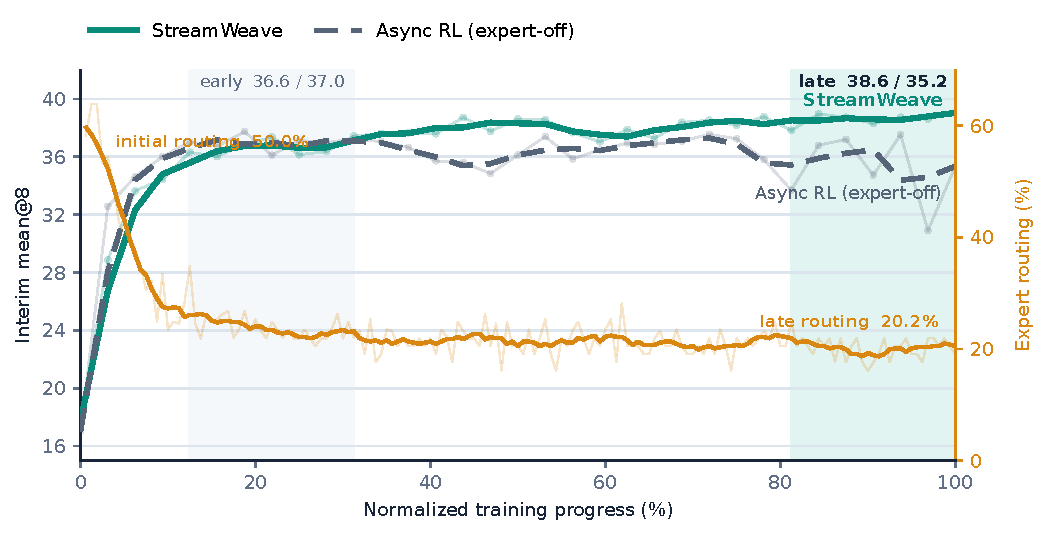
\includegraphics[width=0.84\textwidth]{learning_effect_dynamics.pdf}
  \caption{Learning dynamics over normalized training progress.
  Lines compare interim six-benchmark performance for StreamWeave and the expert-off control; the secondary curve shows expert-routing rate.
  Thin curves are observations, thick curves are smoothed trends, and shaded regions mark the reported early and late windows.}
  \label{fig:learning-dynamics}
\end{figure*}

Expert routing falls rapidly as the policy improves early in training and then settles into a persistent tail, as shown in Figure~\ref{fig:learning-dynamics}.
The required range of supervision narrows, but a residual region without policy-generated signal remains late in training.
This changing use of the expert source is continually incorporated into the same fully-asynchronous training stream as policy rollouts.

StreamWeave and the expert-off control share the execution stack, policy objective, optimizer, prompt population, and expert access; they differ in whether the expert input selected by an all-failure outcome is consumed.
Because such a group supplies no reward-derived relative direction, the expert-off run can reach this region only through transfer from other prompts.
The runs improve similarly at first and then separate, with the same direction appearing in both average benchmark performance and the held-out all-failure rate.

After matching the same prompt and its initial number of successes, StreamWeave obtains higher subsequent performance in all nine strata $k=0,\ldots,8$, with the largest gaps in the partial-success region.
The pattern is consistent with selective expert contributions supporting both the paired prompt and broader acquisition and retention in the shared policy.
Appendix C.3 reports the full stratified results, uncertainty, and later encounters, showing that the pattern extends beyond directly routed prompts while limiting the evidence to a matched longitudinal comparison.

\paragraph{Cross-domain reasoning.}
To test whether math-focused selective expert supervision narrows broader reasoning, we evaluate the same checkpoints on ARC-Challenge, GPQA-Diamond, and MMLU-Pro.

\begin{table}[!htbp]
\centering
\begin{tabular}{@{}lrrrr@{}}
\toprule
Model & ARC-C & GPQA-D & \shortstack{MMLU-\\Pro} & \textbf{Avg.} \\
\midrule
Base & 5.7 & 3.6 & 3.3 & \textbf{4.2} \\
Instruct & 54.6 & 27.7 & 30.3 & \textbf{37.5} \\
\shortstack[l]{Async RL\\(expert-off)} & \textbf{60.8} & \textbf{30.6} & 31.7 & \textbf{41.1} \\
HPT (sync) & 60.5 & 28.8 & 33.9 & \textbf{41.1} \\
SRFT & 48.0 & 24.2 & 28.0 & \textbf{33.4} \\
ReLIFT & 52.8 & 24.5 & 30.2 & \textbf{35.8} \\
Oat-Zero & 41.9 & 13.5 & 21.5 & \textbf{25.6} \\
LUFFY & 56.5 & 27.0 & \textbf{34.5} & \textbf{39.3} \\
\textbf{StreamWeave} & 60.2 & 30.3 & 33.2 & \textbf{41.2} \\
\bottomrule
\end{tabular}
\caption{Fixed-checkpoint cross-domain reasoning; Avg.\ is the unweighted mean.}
\label{tab:cross-domain}
\end{table}

StreamWeave matches the aggregate cross-domain performance of Async RL (expert-off) and HPT (sync), with individual scores remaining within their range, while achieving stronger mathematical reasoning.
The additional learning gain is therefore concentrated in the target mathematical domain without a clear reduction in cross-domain reasoning.

\subsection{Execution Efficiency with Expert Supervision}
\label{sec:execution-efficiency}

\begin{figure*}[!t]
  \centering
  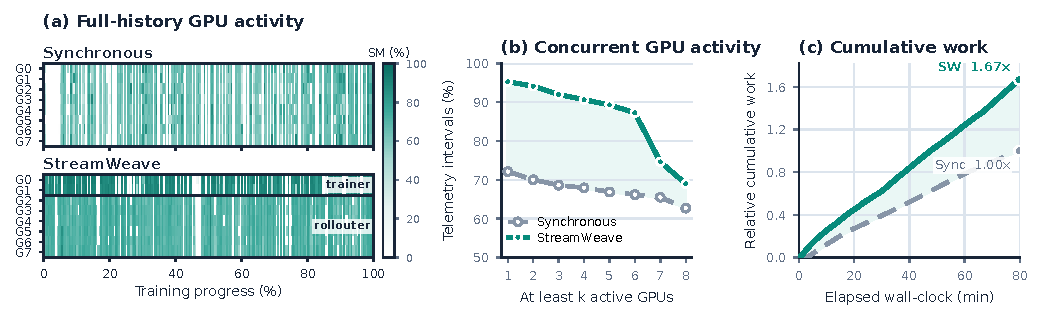
\includegraphics[width=0.94\textwidth]{execution_gpu_activity_overview.pdf}
  \caption{GPU activity and cumulative work under the same 8-GPU budget.
  Panels (a)--(b) independently normalize each run's non-validation history; panel (c) compares the complete synchronous run with an equal-length StreamWeave prefix, normalized to the synchronous endpoint.}
  \label{fig:execution-efficiency}
\end{figure*}

Because the expert source remains part of the online stream throughout training, its accompanying generation workload and group-completion pattern are persistent execution conditions for the fully-asynchronous system.
The question for this section is whether those conditions force the complete-group decision to constrain the rest of the pipeline.

Compared with the expert-off control on the same fully-asynchronous stack, the expert-supervised run produces longer responses and group tails, increasing the incidence of groups containing rollouts from adjacent policy versions (Table~\ref{tab:execution}).

\begin{table}[!htbp]
\centering
\begin{tabular}{@{}lrrr@{}}
\toprule
Metric & Ref. & \textbf{Ours} & Change \\
\midrule
\multicolumn{4}{@{}l}{\textit{Generation workload (expert-off reference)}} \\
Response length (tokens) & 896 & \textbf{1,429} & \textbf{$1.59\times$} \\
Longest rollout/group (s) & 6.59 & \textbf{12.79} & \textbf{$1.94\times$} \\
Adjacent-version groups & 2.03\% & \textbf{7.00\%} & \textbf{$3.46\times$} \\
\midrule
\multicolumn{4}{@{}l}{\textit{End-to-end execution (synchronous reference)}} \\
128-group time (s) $\downarrow$ & 46.0 & \textbf{28.0} & \textbf{$-39\%$} \\
Throughput (groups/s) $\uparrow$ & 2.78 & \textbf{4.58} & \textbf{$1.64\times$} \\
\bottomrule
\end{tabular}
\caption{Generation workload and execution efficiency.
The synchronous reference uses the same GPU budget; all metrics use pre-routing prompt groups as the work unit.}
\label{tab:execution}
\end{table}

This temporal exposure is not uniform across group outcomes.
Within StreamWeave, 10.0\% of the all-failure groups ultimately assigned to the expert source contain rollouts from adjacent policy versions, the highest rate among the routes.
The region that requires an expert source therefore interacts most strongly with asynchronous execution not only through its missing learning signal, but also through when its complete group becomes available.

When all rollouts in a long and uneven group share one execution phase, the slowest trajectory governs pipeline progress.
In the synchronous trace, requests complete in 7.6 seconds on average, but the slowest lasts 23.7 seconds and the generation phase, including post-processing, ends at 25.1 seconds.
Earlier completions cannot launch the next attempt before the phase closes, and model training starts only after generation.
The completion tail therefore constrains both subsequent rollout work and training.

StreamWeave instead refills each rollout slot as soon as an attempt completes.
It preserves group identity and per-rollout generation policy across these independent completions and reconstructs the group only for its source decision.
Other groups continue generating and ready data continue training while a group remains incomplete.
The required coordination therefore ends at the decision and input-construction boundaries rather than propagating into pipeline-wide waiting.

Figure~\ref{fig:execution-efficiency} shows the hardware-level signature of this design: StreamWeave reduces globally low-activity intervals, sustains broader concurrent GPU activity, and accumulates more prompt-group work over the same wall-clock interval.
This connects the bounded scope of complete-group waiting to realized work.

StreamWeave reduces the processing time for 128 prompt groups from 46 to 28 seconds and achieves \textbf{$1.64\times$ full-history prompt-group throughput} under the same GPU budget.
Two connected execution effects contribute to this end-to-end gain.
First, model training that follows generation in synchronous execution proceeds concurrently with rollout generation.
Second, immediately refilling a rollout slot after an attempt finishes recovers capacity that would otherwise be lost while early rollouts wait for the complete-group tail.
Together, these effects retain the complete-group decision while reducing how far its waiting constrains model training and other rollout slots.

Appendices C.4 and C.5 check this interpretation with resource-normalized accounting, source-specific policy-version composition, and request-level timing, while delimiting it as critical-path accounting rather than an exact additive decomposition.

\FloatBarrier
\section{Conclusion}
\label{sec:conclusion}

StreamWeave realizes group-conditioned RLVR under fully-asynchronous execution by separating trajectory execution from the complete-group decision that selects the training source and learning role.
The wait for that decision ends where the source is fixed, and the information that reproduces the selected role ends where the training input is built.
Localizing these dependencies retains the complete group as a learning-decision boundary while separating its completion from a pipeline-wide execution barrier.

Experiments show that all-failure groups carry disproportionately high generation work, demand for the expert source persists late into training, and selective expert contributions relate to acquisition and retention beyond directly routed prompts.
StreamWeave achieves mathematical reasoning performance comparable to the synchronous quality reference and retains competitive cross-domain reasoning.
Even under the longer generation workload observed in the expert-supervised run, it improves prompt-group throughput by $1.64\times$ under the same GPU budget.
Our direct empirical scope is one backbone, one training seed, an 8-GPU budget, and math-centered group-conditioned two-source RLVR.
Within this scope, StreamWeave preserves complete-group learning composition, bounds the execution scope of its dependencies, and combines selective expert supervision with the efficiency of fully-asynchronous execution in one training system.

\bibliography{references}

\end{document}
